\section{Tutorium 17.04.25}
\label{sec:17_04_25}

\subsection{Wiederholung - Komplexe Zahlen}
Mit Sicherheit erinnert ihr euch noch gut an die komplexen Zahlen:
\begin{definition}{Komplexe Zahlen}{komplexezahlen}
Der Körper $(\C, +, \cdot)$ mit
\begin{equation}
\C := \{(a,b) \in \R \mid a,b \in \R\}
\end{equation}
und den Operationen
\begin{equation}
\begin{split}
+: \C \times \C &\to \C\\
(a,b), (c,d) &\mapsto (a,b) + (c,d) := (a+c,b+d),
\end{split}
\end{equation}
genannt Addition, und
\begin{equation}
\begin{split}
\cdot: \C \times \C &\to \C\\
(a,b),(c,d) &\mapsto (a,b) \cdot (c,d) := (ac-bd, ad+bc),
\end{split}
\end{equation}
genannt Multiplikation, nennen wir den Körper der \textbf{komplexen Zahlen}. Die Zahl $a=\Re(a,b)$ heißt \textbf{Realteil}, die Zahl $b=\Im(a,b)$ \textbf{Imaginärteil} von $z$. 
\end{definition}
Meist führt man die \textit{komplexe Einheit} $i$ ein, sodass $(a,b)=a+bi$ für $i^2:=-1$ gilt. Dies erleichtert Rechnungen, ist aber rein symbolischer Natur. Fundamental ist, dass hier ein Körper vorliegt: Sowohl $(\C, +)$ als auch $(\C^\ast, \cdot)$ sind Gruppen (das könnt ihr gerne zur Übung nachprüfen, vor allem die Inversen sollte man einmal konstruiert haben). Bereits aus MfP1 kennt ihr die \textit{komplexe Konjugation}
\begin{equation}
\begin{split}
\overline{\cdot}: \C &\to \C\\
z = a+bi &\mapsto \overline{z} := a-bi.
\end{split}
\end{equation}
Geometrisch entspricht dies einer Spiegelung an der reellen Achse. Auf $\C$ definieren wir außerdem den \textit{Absolutwert} oder \textit{Betrag} durch
\begin{equation}
\begin{split}
|\cdot |: \C &\to \C\\
z &\mapsto |z| := \sqrt{z \overline{z}} = \sqrt{\Re(z)^2+\Im(z)^2}
\end{split}
\end{equation}
mit einigen wichtigen Eigenschaften:
\begin{enumerate}[({M}1)]
\item Positivität: $|z| \geq 0$ mit $|z| = 0 \iff z=0$
\item Multiplikativität: $|z_1z_2| = |z_1||z_2|$
\item Subadditivität (Dreiecksungleichung): $|z_1+z_2| \leq |z_1| + |z_2|$.
\end{enumerate}
Sowohl die Multiplikativität als auch die Subadditivität kann man induktiv auf beliebige \red{endliche} Produkte bzw. Summen ausweiten.\\
Damit erhalten wir eine Möglichkeit, aus geometrischen Überlegungen verschiedene Formen für komplexe Zahlen herzuleiten. Ausgehend von der \textit{kartesischen Form} $z=a+bi$ definieren wir den \textbf{Radius} von $z$ als $r := |z|$. Das \textbf{(Haupt-)Argument} von $z$ ist dessen eingeschränkter Polarwinkel $\phi \in (-\pi, \pi]$, das aus trigonometrischen Überlegungen hergeleitet werden kann. Damit erhalten wir die \textit{Polarform} und mit der Eulerschen Formel auch die \textit{trigonometrische Form}:
\begin{equation}
z = r \exp(i\phi) = r(\cos \phi + i \sin \phi).
\end{equation} 
\begin{figure}[H]
\centering
\begin{tikzpicture}[scale=3]
	\draw[step=.5cm, gray, very thin, dotted] (-1.4,-1.4) grid (1.4,1.4);
	\foreach \x/\xtext in {-1, 1}
		\draw (\x,-1pt) -- (\x, 1pt) node[anchor=north] {$\xtext$};
	\foreach \y/\ytext in {-1, 1}
		\draw (-1pt, \y) -- (1pt, \y) node[anchor=east, left=2pt] {$\ytext$};
	\draw[->] (-1.5,0) -- (1.5,0);
	\draw[->] (0,-1.5) -- (0,1.5);
	\draw (0,0) circle [radius=1cm];
	\draw (.5cm,0) arc [start angle=0, end angle=40, radius=.5cm] node[right=1pt,pos=0.5] {$\phi$};
	\draw[red] (40:1cm) -- node[right=1pt, thick] {$\sin \phi = \Im(z)$} (40:1cm |- 0,0);
	\draw[blue] (0,0) -- node[below=4pt,pos=0.5, thick] {$\cos \phi = \Re(z)$} (40:1cm |- 0,0);
	\draw (0,0) -- node[above=2pt, thick] {$r$}  (40:1cm) node[black, right=1pt] {$z$};
	\filldraw[black] (40:1cm) circle [radius=0.5pt];
\end{tikzpicture}
\caption{Die Einheitskreislinie $\S^1 \hookrightarrow \C$ mit der komplexen Zahl $z=r\exp(i\phi)$.}
\end{figure}
Nicht immer ist es ganz so einfach, das Argument aus der kartesischen Form zu ermitteln. Wir illustrieren dies mal wie folgt:
\begin{figure}[H]
\centering
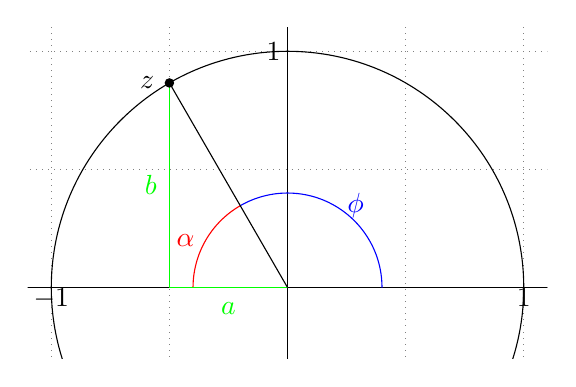
\begin{tikzpicture}[scale=3]
	\clip (-1.1, -0.3) rectangle (1.1, 1.1);
	\draw[step=.5cm, gray, very thin, dotted] (-1.4,-1.4) grid (1.4,1.4);
	\foreach \x/\xtext in {-1, 1}
		\draw (\x,-1pt) -- (\x, 1pt) node[anchor=north] {$\xtext$};
	\foreach \y/\ytext in {-1, 1}
		\draw (-1pt, \y) -- (1pt, \y) node[anchor=east, left=2pt] {$\ytext$};
	\draw[->] (-1.5,0) -- (1.5,0);
	\draw[->] (0,-1.5) -- (0,1.5);
	\draw (0,0) circle [radius=1cm];
	\draw[blue] (.4cm,0) arc [start angle=0, end angle=120, radius=.4cm] node[right=1pt,pos=0.5] {$\phi$};
	\draw[red] (-.4cm,0) arc [start angle=180, end angle=120, radius=.4cm] node[left=.5pt, pos=0.5] {$\alpha$};
	\draw[green] (120:1cm) --  (120:1cm |- 0,0) node[left=1pt,pos=0.5] {$b$} ;
	\draw[green] (0,0) -- node[below=2pt] {$a$} (120:1cm |- 0,0) ;
	\draw (0,0) --   (120:1cm) node[black, left=2pt] {$z$};
	\filldraw[black] (120:1cm) circle [radius=0.5pt];
\end{tikzpicture}
\caption{In diesem Fall lässt sich der Polarwinkel von $z=a+ib$ nicht direkt ableiten. Wir erhalten $\cos \alpha = \frac{|a|}{\sqrt{a^2+b^2}}$ und damit $\phi = \pi - \arccos(\frac{|a|}{\sqrt{a^2+b^2}}) = \arccos(\frac{a}{\sqrt{a^2+b^2}})$. Dabei nutzt man, dass $\arccos(x) = \pi - \arccos(-x)$ gilt.}
\end{figure}
Wir wollen nun die wichtigen topologischen Begriffe auf $\C$ betrachten. Die Topologie der komplexen Ebene wird von der Metrik induziert:
\begin{definition}{Topologie auf $\C$}{epsilonball}
Der \textbf{offene $\epsilon$-Ball} in $\C$ ist die Teilmenge 
\begin{equation}
B_\epsilon(z) := \{x \in \C \mid |z-x| < \epsilon\}
\end{equation}
mit Radius $\epsilon$ und Mittelpunkt $z$. Eine Teilmenge $X \sub \C$ ist genau dann offen, wenn für alle $z \in X$ gilt, dass $B_\epsilon(z) \sub X$ für ein $\epsilon>0$ erfüllt ist.
\end{definition}
Man erinnere sich daran, dass eine abgeschlossene Menge darauf aufbauend definiert ist: Eine Teilmenge $A \sub \C$ heißt \textit{abgeschlossen}, wenn ihr Komplement $\C \setminus A$ offen ist. Eine Menge kann sowohl abgeschlossen als auch offen sein. Wir brauchen noch weitere Grundbegriffe der Topologie:
\begin{definition}{Zusammenhang und Gebiet}{gebiet}
\begin{enumerate}[(i)]
\item Eine Teilmenge $A \sub \C$ heißt \textbf{zusammenhängend}, wenn sie sich nicht in zwei \textcolor{red}{offene, disjunkte, nicht-leere} Teilmengen zerlegen lässt. Äquivalent dazu ist, dass bei einer Zerlegung $A = B \cup C$ mit $B,C$ offen und disjunkt $A$ oder $B$ die leere Menge sein muss.
\item Eine Teilmenge $A \sub \C$ heißt \textbf{Gebiet}, wenn sie zusammenhängend, offen und nicht-leer ist.
\end{enumerate}
\end{definition}

Mit diesem Wissen sollte es uns leichter fallen, Teilmengen von $\C$ zu charakterisieren. Das versuchen wir zur Übung gleich einmal:
\begin{übung}
Skizziere folgende Teilmengen von $\C$:
\begin{enumerate}[(a)]
\item $M_1 := \{z \in \C \mid 3 \leq |z| \leq 10 \}$
\item $M_2 := \{z \in \C \mid \Re(z^2) > 0 \}$
\item $M_3 := \{z \in \C^\ast \mid \Re \left( \frac{1}{z}\right) \leq 2\}$
\end{enumerate}
Entscheide außerdem, ob die angegebenen Mengen Gebiete (in der von der Metrik induzierten Topologie) sind.
\end{übung}
\begin{lösung}
\begin{enumerate}[(a)]
\item Hier hat man wahrscheinlich schon ein Bild vor Augen, denn wenn man die Polardarstellung $z=r\exp(i \phi)$ einsetzt, erhält man unmittelbar 
\begin{equation}
	3 \leq |r| \leq 10,
\end{equation}
da $|\exp(i \phi)|=1$. Wir erhalten also einen \textit{Kreisring}, wie unten abgebildet. Die Menge ist außerdem offensichtlich nicht offen, denn jeder Randpunkt $z \in \partial M_1$ besitzt keinen offenen $\epsilon$-Ball $B_\epsilon(z)$, der noch ganz in $M_1$ liegt. Also kann $M_1$ kein Gebiet sein.
\item Wir setzen $z=a+bi$ an und erhalten die Ungleichung 
\begin{equation}
\Re((a+bi)^2) = \Re(a^2-b^2+2iab)=a^2-b^2 >0.
\end{equation}
Dies ist äquivalent zu $a^2 > b^2$, die Menge wird also nach unten beschränkt durch die Raumdiagonalen $\Delta_{(a,a)}$ und $\Delta_{(a,-a)}$. Wir erhalten den Longitudinalschnitt eines Kegels, wobei der Ursprung ausgenommen wird. Diese Menge ist offen, denn für alle $z \in M_2$ liegt der offene $\epsilon$-Ball mit $\epsilon<\frac{a}{2}$ für beliebiges $a$ auf der Diagonale noch ganz in $M_2$. Jedoch ist die Menge kein Gebiet, da sie nicht zusammenhängend ist.
\item Wir setzen erneut $z=a+bi$ an und machen folgende Feststellung:
\begin{equation}
\frac{1}{z}=\frac{1}{a+bi}=\frac{a-bi}{(a+bi)(a-bi)}=\frac{a}{a^2+b^2} - i \frac{b}{a^2+b^2}.
\end{equation}
Also ist die Ungleichung durch 
\begin{equation}
\frac{a}{a^2+b^2} \leq 2 \iff 0 \leq a^2 - \frac{a}{2} +b^2
\end{equation}
gegeben. Quadratische Ergänzung liefert
\begin{equation}
0 \leq \left( a - \frac{1}{4} \right)^2 - \frac{1}{16} + b^2 \iff \left( \frac{1}{4} \right)^2 \leq \left( a - \frac{1}{4} \right)^2 +b^2,
\end{equation}
was gerade die Gleichung eines Kreises mit Radius $\frac{1}{4}$ darstellt, der auf $\left( \frac{1}{4},0\right)$ zentriert ist. Man sollte beachten, dass die Ungleichung so gestellt ist, dass die Menge ganz $\C$ ohne den Inhalt des Kreises darstellt. Dies ist aus den gleichen Gründen wie für $M_1$ kein Gebiet, denn die Punkte auf der Kreislinie haben keine offene Umgebung in $M_3$.
\end{enumerate}
\begin{figure}[H]
\centering
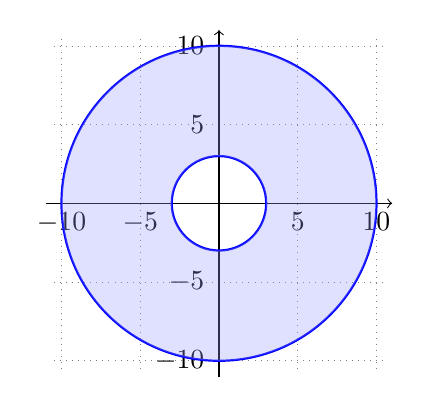
\begin{tikzpicture}[scale=.2]
	\draw[step=5cm, gray, very thin, dotted] (-10.5,-10.5) grid (10.5,10.5);
	\foreach \x/\xtext in {-10,-5,5,10}
		\draw (\x,-1pt) -- (\x, 1pt) node[anchor=north] {$\xtext$};
	\foreach \y/\ytext in {-10,-5,5,10}
		\draw (-1pt, \y) -- (1pt, \y) node[anchor=east, left=2pt] {$\ytext$};
	\draw[->] (-11,0) -- (11,0);
	\draw[->] (0,-11) -- (0,11);
	\draw[thick, blue] (0,0) circle [radius=3];
	\draw[thick, blue] (0,0) circle [radius=10];
	\fill[blue!40, opacity=.3, even odd rule] (0,0) circle [radius=3] (0,0) circle [radius=10];
\end{tikzpicture}
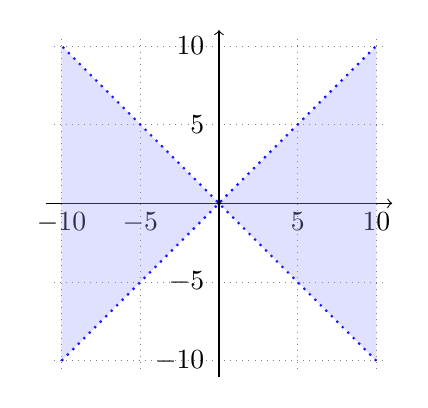
\begin{tikzpicture}[scale=.2]
	\draw[step=5cm, gray, very thin, dotted] (-10.5,-10.5) grid (10.5,10.5);
	\foreach \x/\xtext in {-10,-5,5,10}
		\draw (\x,-1pt) -- (\x, 1pt) node[anchor=north] {$\xtext$};
	\foreach \y/\ytext in {-10,-5,5,10}
		\draw (-1pt, \y) -- (1pt, \y) node[anchor=east, left=2pt] {$\ytext$};
	\draw[->] (-11,0) -- (11,0);
	\draw[->] (0,-11) -- (0,11);
	\draw[thick, blue, dotted] (-10,-10) -- (10,10);
	\draw[thick, blue, dotted] (10,-10) -- (-10,10);
	\fill[blue!40, opacity=.3] (0,0) -- (10,-10) -- (10,10) -- cycle;
	\fill[blue!40, opacity=.3] (0,0) -- (-10,-10) -- (-10,10) -- cycle;
	\filldraw[black] (0,0) circle (.1);
\end{tikzpicture}
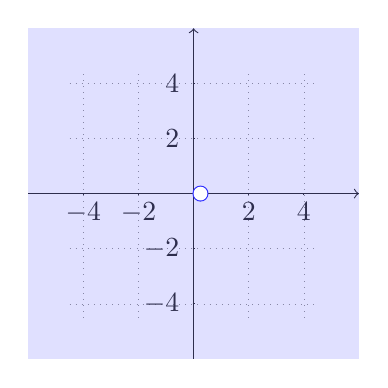
\begin{tikzpicture}[scale=.35]
	\draw[step=2cm, gray, very thin, dotted] (-4.5,-4.5) grid (4.5,4.5);
	\foreach \x/\xtext in {-4,-2,2,4}
		\draw (\x,-1pt) -- (\x, 1pt) node[anchor=north] {$\xtext$};
	\foreach \y/\ytext in {-4,-2,2,4}
		\draw (-1pt, \y) -- (1pt, \y) node[anchor=east, left=2pt] {$\ytext$};
	\draw[->] (-6,0) -- (6,0);
	\draw[->] (0,-6) -- (0,6);
	\draw[thick, blue] (0.25,0) circle [radius=0.25];
	\fill[blue!40, opacity=.3] (-6,-6) rectangle (6,6);
	\fill[white] (.25,0) circle (.25);
\end{tikzpicture}
\end{figure}
\end{lösung}
Eine weitere sehr wichtige Ungleichung wollen wir zur Übung beweisen:
\begin{satz}{Cauchy-Schwarz-Ungleichung}{cauchyschwarz}
Seien $x_1, \dots, x_n, y_1, \dots, y_n \in \C$ endlich viele komplexe Zahlen. Dann gilt die \textbf{Cauchy-Schwarz-Ungleichung}
\begin{equation}
\left| \sum_{i=1}^n x_i \overline{y}_i\right|^2 \leq \sum_{i=1}^n |x_i|^2 \sum_{i=1}^n |y_i|^2.
\end{equation}
\end{satz}
\begin{beweis}
Für den Beweis brauchen wir zwei Vorüberlegungen. Erst einmal bemerken wir, dass die Gleichung immer gilt, wenn $\sum_i |x_i|^2 \sum_i|y_i|^2 = 0$, da dann alle $x_i$ oder alle $y_i$ verschwinden müssen. Wir müssen den Beweis also nur noch für $\sum_i |x_i|^2 \sum_i|y_i|^2 > 0$ führen. Die andere Vorüberlegung ist etwas technisch\footnote{Wer denkt, die folgenden Umformungen fielen vom Himmel, kann versuchen, es von vorn nach hinten anzugehen. Dann ist es viel offensichtlicher.} Seien $\alpha, \beta, \gamma, \delta \in \R$. Da Quadrate reeller Zahlen immer positiv sind, stellen wir fest:
\begin{align*}
0 \leq (\alpha \delta- \beta \gamma)^2 &= \alpha^2\delta^2 + \beta^2 \gamma^2 -2\alpha \beta \gamma \delta\\
&= \blue{\alpha^2 \beta^2 - \alpha^2 \beta^2 + \gamma^2 \delta^2 - \gamma^2 \delta^2} +\alpha^2\delta^2 + \beta^2 \gamma^2 -2\alpha \beta \gamma \delta\\
&= (\alpha^2 + \gamma^2)(\beta^2+\delta^2) - (\alpha^2 \beta^2 + \gamma^2 \delta^2 + 2 \alpha \beta \gamma \delta)\\
&= (\alpha^2 + \gamma^2)(\beta^2+\delta^2) - (\alpha \beta + \gamma \delta)^2.
\end{align*}
Umstellen liefert nun eine Ungleichung, derer wir uns später bedienen:
\begin{equation}
(\ast)\, (\alpha \beta + \gamma \delta)^2 \leq (\alpha^2 + \gamma^2)(\beta^2+\delta^2).
\end{equation}
Nun beweisen wir endlich die Ungleichung mit vollständiger Induktion:\\
Für den Induktionsanfang brauchen wir nur (M2):
\begin{equation}
|x\overline{y}|^2 = (|x||\overline{y}|)^2 = |x|^2|y|^2.
\end{equation}
Hier gilt sogar Gleichheit. Die Induktionsvoraussetzung (IV) ist, dass die Aussage für $n-1$ gezeigt ist. Da beide Seiten positiv sind, können wir in der IV die Wurzel ziehen:
\begin{equation}
\left| \sum_{i=1}^{n-1} x_i \overline{y}_i\right| \leq \sqrt{\sum_{i=1}^{n-1} |x_i|^2} \sqrt{\sum_{i=1}^{n-1} |y_i|^2}.
\end{equation}
Für den Induktionsschritt müssen wir die Aussage für $n$ beweisen. Das geht nun relativ schnell:
\begin{align*}
\left| \sum_{i=1}^n x_i \overline{y}_i\right| &= \left| x_n \overline{y}_n + \sum_{i=1}^{n-1} x_i \overline{y}_i\right|\leq |x_n \overline{y}_n| + \left| \sum_{i=1}^{n-1} x_i \overline{y}_i\right|\\
&\leq^\text{\red{IV}} |x_n| |y_n| + \sqrt{\sum_{i=1}^{n-1} |x_i|^2} \sqrt{\sum_{i=1}^{n-1} |y_i|^2} \leq^{\red{(\ast)}} \sqrt{\sum_{i=1}^{n} |x_i|^2} \sqrt{\sum_{i=1}^{n} |y_i|^2}
\end{align*}
Im ersten Schritt haben wir die Dreiecksungleichung ausgenutzt, gefolgt von der Induktionsvoraussetzung. Den letzten Schritt können wir mit unserer Ungleichung $(\ast)$ direkt folgern, indem wir $\alpha:=|x_n|$, $\beta:= |y_n|$, $\gamma:= \sqrt{\sum_{i=1}^{n-1} |x_i|^2}$ und $\delta :=\sqrt{\sum_{i=1}^{n-1} |y_i|^2}$ setzen.
\end{beweis}